\chapter{Imagen Digital}

Existen dos tipos de im�genes utilizadas frecuentemente en visi�n por computador: Im�genes de intensidad e im�genes de alcance.

Las im�genes de alcance, tambi�n denominadas im�genes o mapas de profundidad, tiene su fundamento en los sensores de alcance �pticos y estiman directamente la estructura de la imagen en tres dimensiones de la escena.
Las im�genes de intensidad miden la cantidad de luz que incide en un dispositivo fotosensible. Es este tipo de im�genes sobre las cuales hemos trabajado en nuestro proyecto.

Las estructuras de datos utilizadas en la digitalizaci�n de una imagen son varias:
\begin{itemize}
\item Tradicionales
\begin{enumerate}
\item Matrices
\item Cadenas
\item Estructuras topol�gicas
\item Estructuras relacionales
\end{enumerate} 
\item Jer�rquicas
\begin{enumerate}
\item Pir�mides
\item Quadtrees
\end{enumerate} 
\end{itemize} 

Las que nosotros hemos utilizado han sido matrices, es decir, una imagen digitalizada formar�a una matriz tal que:
\begin{center}
f(x,y) \equiv valor proporcional a la intensidad de luz en el punto (x,y)

\includegraphics[scale=1]{rob1.png} 
\end{center} 
	
Cada elemento de la matriz o p�xel tendr� un valor asignado que se corresponde con el nivel de luminosidad del punto correspondiente en la escena captada, dicho valor es el resultado de la cuantizaci�n de intensidad o nivel de gris.
Se suele utilizar el termino bitmap para hacer referencia a un mapa de p�xeles, aunque en algunos ambientes se preserva para aquellos mapas de p�xeles en los que un p�xel se representa por un simple bit.

Si la imagen es en blanco y negro, se almacena solo un valor por p�xel, en nuestro caso las im�genes son a color, lo que hace que los elementos de la matriz ya no tengan asociado un solo valor sino tres, correspondientes el rojo, verde y azul. 
A este modelo se le llama modelo de color RGB.
Cada valor de p�xel es un triple ordenado (r, g, b), donde r, g, b representan las intensidades de rojo ,verde y azul respectivamente. r, g, b son cadenas de bits, en nuestro caso, son de 8 bits, esto significa que el rango de valores var�a de 0 a 255, donde el 0 representa el negro absoluto y el 255 el blanco absoluto.

Algunas correspondencias de colores en el modelo RGB son:
\begin{itemize}
\item Negro:	(0,0,0)
\item Azul:	(0,0,255)
\item Verde:	(0,255,0)
\item Rojo:	(255,0,0)
\item Amarillo:	(255,255,0)
\item Blanco:	(255,255,255)
\end{itemize} 
	
La profundidad del color se define como la suma de los bits asociados a los componentes r, g, b. Por ejemplo, si utilizamos 2 bits para el rojo, 2 para el verde y 2 para el azul, tendremos una profundidad de color de 6 bits por p�xel, y una paleta de colores de 2^{6} = 64 posibles colores.
La profundidad de color ideal es la de 24 bits por p�xel, conocida como color verdadero. Por encima de esta profundidad el ojo humano es incapaz de notar la diferencia.

Dos factores que afectan a la calidad de una imagen es su resoluci�n espacial y en amplitud. Dependiendo del numero de pixels que tenga el dispositivo la imagen poseer� mas o menos resoluci�n espacial. Y la amplitud se refiere al rango de bits destinados para representar la intensidad de cada p�xel. 
A mas resoluci�n en ambos campos mas memoria se requiere, pero mas n�tida es la imagen. Un ejemplo de un gr�fico a color verdadero con una resoluci�n de 1280 x 1024, necesita:

\begin{center}
1280 x 1024 x 24 = 31457280 bits (casi 4 Mb)
\end{center} 
 	 
\begin{center}
\begin{tabular}{|c|c|}
\hline 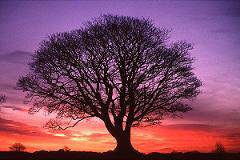
\includegraphics[scale=1]{arbol1.png}  & 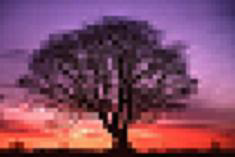
\includegraphics[scale=1]{arbol2.png}  \\ 
\hline 
\end{tabular} 
Dos representaciones de la misma imagen con la variaci�n del numero de pixels utilizados.
La de la izquierda tiene una resoluci�n de 240x160 y la de la derecha de 48x32.
\end{center} 

\begin{center}
\begin{tabular}{|c|c|}
\hline 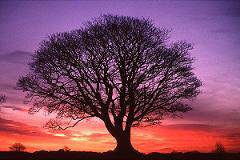
\includegraphics[scale=1]{arbol1.png}  & 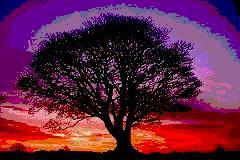
\includegraphics[scale=1]{arbol3.png}  \\ 
\hline 
\end{tabular} 
Dos representaciones de la misma imagen con variaci�n en el numero de niveles de color utilizados. La de la izquierda posee 256 y la de la derecha 8.
\end{center} 	 

Resumiendo, el termino imagen se refiere a una funci�n de intensidad bidimensional f(x,y), donde x, y son las coordenadas espaciales y el valor de f en cualquier punto (x, y) es proporcional a la intensidad de color.
Una vez que se tiene definido el sistema de ejes cartesianos, ya es posible realizar cualquier tipo de operaci�n. Estas operaciones ser�n los filtros, que aplicados sobre la imagen la modificaran. 

